
\section{羟基酸}

羟基酸的特别点一般在于其发生酯化反应时的特性。

\subsection{交酯}

两分子α-羟基酸相互发生分子间酯化形成的六元环状二酯。其中一分子羟基酸的羟基 $\ce{-OH}$ 与另一分子羟基酸的羧基 $\ce{-COOH}$ 缩合脱去一分子水生成酯,同时这一分子羟基酸的羧基 $\ce{-COOH}$ 又与另一分子羟基酸的羟基 \ce{-OH} 缩合生成另一个酯基。

\begin{figure}[h]
    \centering
    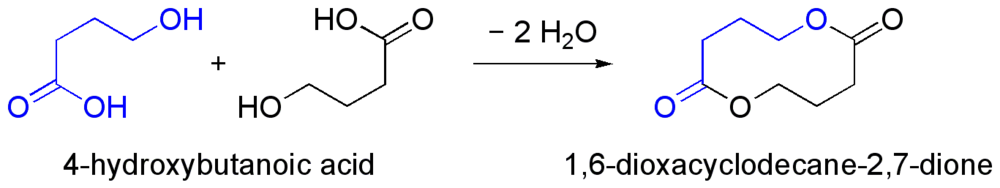
\includegraphics[width=0.8\textwidth]{img/1000px-hydroxybutanoic.png}
\end{figure}

\subsection{缩聚}

高中学的那个缩聚反应。


\subsection{降解反应}
